\section{Needleman–Wunsch}
\label{sec:needleman-wunsch}
\newcommand{\lenn}{\text{len}}

The Needleman–Wunsch algorithm calculates the global alignment of two strings and was originally used in bio-informatics to compare amino acid sequences of two proteins \cite{nw}. For our purposes, the alphabet will instead consist of the phonetic \gls{ipa} symbols. Out of all possible alignments of two words (including gaps), the Needleman–Wunsch algorithm finds the one with the smallest distance, \ie the alignment with the highest \q{score}. The algorithm is based on dynamic programming and has a time complexity of $\mathcal{O}(\lenn(A) \cdot \lenn(B))$, where $A$ and $B$ are the two words to be compared.

\autoref{alg:needleman-wunsch} features the pseudo-code of the score computation\footnote{The respective \href{https://en.wikipedia.org/wiki/Needleman\%E2\%80\%93Wunsch_algorithm}{Wikipedia page} also provides a good introduction. Furthermore, the score matrix is interactively explained in \cite{nw_demo}.}. In \autoref{fig:matrix-nuance-puissance-optimal}, we see the resulting score matrix that the algorithm constructed for the French words \textit{puissance} and \textit{nuance}. Follow the indicated path (red tiles) from the bottom right to the top left to find the (reversed) optimal alignment (see \autoref{tab:nuance-puissance-alignment-optimal}).

\begin{table}[H]
\centering
\begin{tabular}{l*{6}{>{\centering\arraybackslash}p{0.2cm}}}
    \toprule
    \textit{puissance}
    & \textipa{p} & \textipa{\textturnh} & \textipa{i} & \textipa{s} & \textipa{\~A} & \textipa{s}\\
    \midrule
    \textit{nuance}
    & \textipa{n} & \textipa{\textturnh} & -- & -- & \textipa{\~A} & \textipa{s}\\
    \bottomrule
\end{tabular}
\caption{The optimal alignment yields a score of $-2$. See the path in \autoref{fig:matrix-nuance-puissance-optimal}.}
\label{tab:nuance-puissance-alignment-optimal}
\end{table}

\begin{figure}[H]
    \centering
    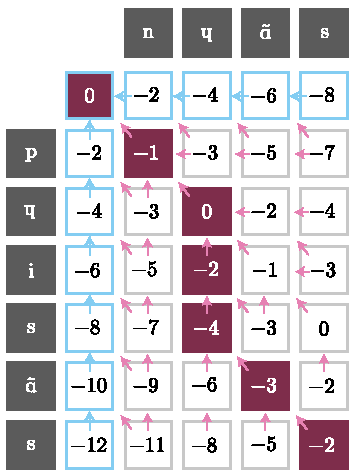
\includegraphics[width=0.77\linewidth]{assets/illustrator/matrix-nuance-puissance-optimal.pdf}
    \caption{Needleman–Wunsch score matrix for the words $A\coloneqq\textit{puissance}$ \textipa{/p\textturnh is\~As/} (power, strength) and $B\coloneqq\textit{nuance}$ \textipa{/n\textturnh\~As/} (nuance, shade). The arrows indicate which steps locally maximize the score. The red tiles trace the path of the optimal alignment. Match Score: $1$, Mismatch Score: $-1$, Gap Penalty: $p=-2$.}
    \label{fig:matrix-nuance-puissance-optimal}
\end{figure}

\vfill\null

We first discuss the meaning of the different steps (arrows) in the score matrix (\autoref{fig:matrix-nuance-puissance-optimal}) to then explain how to construct this matrix.

\begin{itemize}

    \item In a \textbf{diagonal step}, both symbols (which indicate the current position in the two words) change. Such a step corresponds to either a match or mismatch between the two symbols. In the example, the \textipa{/s/} symbols in the bottom-right corner match, which is why the step beforehand is a \textit{diagonal} step from the field $-3$ to $-2$. The score increases by $1$ since we defined the match score to be $+1$.

    \item In a \textbf{vertical} or \textbf{horizontal step}, only one of the two symbols changes. We interpret this as a gap in the alignment, \ie one symbol aligns to a gap in the other word. In the example, this is the case two times when we move from the red field $0$ down to $-2$ and then down to $-4$. The score decreases by $2$ each time, as we defined the gap penalty as $p \coloneqq -2$ in this example. The gap is indicated by \q{--} in the alignment (see \autoref{tab:nuance-puissance-alignment-optimal}). As we are still in the column of \textipa{/\textturnh/} of the word \textipa{/n\textturnh\~As/}, we insert two \q{--} symbols after the \textipa{/\textturnh/}. This step is sometimes also referred to as \textbf{deletion} or \textbf{insertion}.
    
\end{itemize}

To find the score matrix for given input words $A$ and $B$, we follow \autoref{alg:needleman-wunsch}. First, the score matrix of dimension $(\lenn(A)+1) \times (\lenn(B)+1)$ is initialized\footnote{This does not necessarily involve setting all fields to $0$ as will become clear.}. Then, in lines~\ref{algstep:init-gap-start} to~\ref{algstep:init-gap-end}, the blue-bordered tiles of \autoref{fig:matrix-nuance-puissance-optimal} are filled with the gap penalty $p$ times the index. This is necessary since the only possible step for these tiles is either a vertical or horizontal step (blue arrows), thus leading to a gap in the alignment as discussed beforehand. This gap is punished with gap penalty $p$.

\begin{figure}[H]
    \centering
    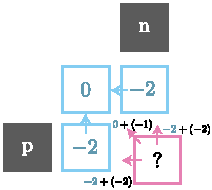
\includegraphics[width=0.6\linewidth]{assets/illustrator/matrix-nuance-puissance-subcalc.pdf}
    \caption{Calculations for one element of the Needleman–Wunsch score matrix.}
    \label{fig:matrix-nuance-puissance-subcalc}
\end{figure}

In the nested loops (lines~\ref{algstep:nested1} and~\ref{algstep:nested2}), we then iterate over the remaining fields of the score matrix (index now starts at $1$, not $0$) which corresponds to traversing the matrix row-wise. To each field, we assign the maximum of three values:

\begin{figure*}

\begin{minipage}[t]{0.6\textwidth}

\begin{algorithm}[H]
    \DontPrintSemicolon
    
    \SetKwFunction{calcScoreFunc}{calculateScore}
    \SetKwData{WordA}{$A$}
    \SetKwData{WordB}{$B$}
    \SetKwData{Sim}{similarity}
    \SetKwData{GapPenalty}{$p$}
    \SetKwData{ScoreMatrix}{scoreMatrix}
    \newcommand{\ScoreMatrixIdx}[2]{{\ScoreMatrix}[{#1}][{#2}]}
    \SetKwData{Cost}{cost}
    \SetKwData{MatchScore}{matchScore}
    \SetKwData{DeleteScore}{deleteScore}
    \SetKwData{InsertScore}{insertScore}
    \SetKwData{Score}{score}
    \SetKwFunction{len}{len}

    \KwIn{
        \small{\!\!\small{$\WordA = \set{A_0, \ldots, A_{\len(A)-1}}$,
        $\WordB = \set{B_0, \ldots, B_{\len(B)-1}}$}},\\
        \qquad\qquad \Sim: \small{similarityScoreFunc},
        \GapPenalty: GapPenalty
    }
    \KwOut{\Score}
    \Fn{\calcScoreFunc{}}
    {
        \SetInd{0.25em}{0.55em}
        Init \ScoreMatrix with dimensions $\small{(\len(\WordA)+1) \times (\len(\WordB)+1)}$\;

        \BlankLine

        \For{$i \in \{0, \ldots, \len(\WordA)\}$\label{algstep:init-gap-start}}
        {
            \ScoreMatrixIdx{$i$}{$0$} $\gets \GapPenalty \cdot i$\;
        }
        \For{$j \in \{0, \ldots, \len(\WordB)\}$}
        {
            \ScoreMatrixIdx{$0$}{$j$} $\gets \GapPenalty \cdot j$
            \label{algstep:init-gap-end}\;
        }

        \BlankLine

        \For{$i \in \{1, \ldots, \len(\WordA)\}$\label{algstep:nested1}}
        {
            \For{$j \in \{1, \ldots, \len(\WordB)\}$\label{algstep:nested2}}
            {
                \Cost $\gets$ $\Sim(\WordA_{i-1}, \WordB_{j-1})$
                \label{algstep:sim}\;
                \MatchScore $\gets$ \ScoreMatrixIdx{$i-1$}{$j-1$} + \Cost
                \label{algstep:matchscore}\;
                \DeleteScore $\gets$ \ScoreMatrixIdx{$i-1$}{$j$} + \GapPenalty
                \label{algstep:deletescore}\;
                \InsertScore $\gets$ \ScoreMatrixIdx{$i$}{$j-1$} + \GapPenalty
                \label{algstep:insertscore}\;
                \ScoreMatrixIdx{$i$}{$j$} $\gets$
                $\max(\MatchScore, \DeleteScore, \InsertScore)$
                \label{algstep:max}\;
            }
        }

        \BlankLine

        \Return\! \ScoreMatrixIdx{$\len(\WordA)$}{$\len(\WordB)$}\;
    }
    
    \caption{Needleman–Wunsch}
    \label{alg:needleman-wunsch}
\end{algorithm}

\end{minipage}%
\hfill
\begin{minipage}[t]{0.35\textwidth}

\begin{figure}[H]
    \centering
    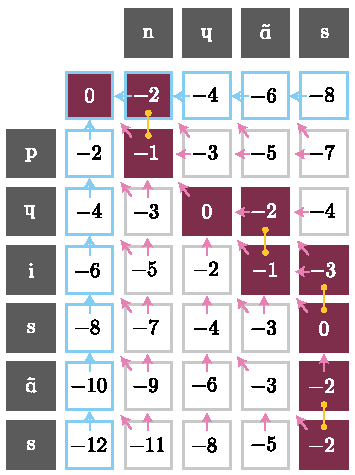
\includegraphics[width=0.87\linewidth]{assets/illustrator/matrix-nuance-puissance-non-optimal.pdf}
    \caption{Needleman–Wunsch score matrix and the path (in red) for a non-optimal alignment. Orange strokes indicate non-optimal steps. Parameters as in \autoref{fig:matrix-nuance-puissance-optimal}.}
    \label{fig:matrix-nuance-puissance-non-optimal}
\end{figure}

\end{minipage}
\end{figure*}

\begin{itemize}[leftmargin=0cm]

    \item The \textbf{match score} is calculated by checking the step to the upper left diagonal (\autoref{algstep:matchscore}). In the example of \autoref{fig:matrix-nuance-puissance-subcalc}, this would result in a value $0+(-1) = -1$, where $0$ is the value in the upper left diagonal field and $-1$ is the cost of the mismatch between \textipa{/p/} and \textipa{/n/}. In case of a match, the new value would be $0 + 1 = 1$. In the algorithm, we also consider the case where costs for a match and a mismatch depend on the symbols themselves, which is why we introduce the function \textit{similarity} that returns the cost of aligning two symbols. This is especially useful when comparing phonetic symbols, as the similarity between two symbols can be defined in a more sophisticated way than just $1$ or $-1$ (\eg replacing a vowel with a consonant might be more costly than replacing a vowel with another vowel). This function might also be represented as a \q{similarity matrix}.
    
    \item The \textbf{delete score} refers to the step from the field above (\autoref{algstep:deletescore}). In the example, we find $(-2) + (-2) = -4$ as new value ($-2$ is the value in the field above and $p=-2$ is the gap penalty). This steps signifies that a symbol in word A aligns to a gap in word B (here: \textipa{/i/} and \textipa{/s/} of \textit{puissance} align to gaps in \textit{nuance}).
    
    \item The \textbf{insert score} refers to the step from the left (\autoref{algstep:insertscore}). In the example, we find $(-2) + (-2) = -4$ as new value ($-2$ is the value in the field to the left and $p=-2$ is the gap penalty). This step signifies that a symbol in word B aligns to a gap in word A (this does not occur in the example).

\end{itemize}

The new value of the current field is assigned the maximum of these values (\autoref{algstep:max}), such that we locally maximize the score: $\max(-1, -4, -4) = -1$. In \autoref{fig:matrix-nuance-puissance-optimal}, we additionally kept track of the steps that led to the optimal alignment by means of the rose arrows (sometimes multiple optimal steps are possible). For our purposes, we don't want to reconstruct the exact alignment that led to the optimal score, but only the score itself. Thus, we can omit the backtracking step and don't need to store the rose arrows.

By construction, \textbf{the bottom-right field of the score matrix contains the score of the optimal alignment}. This is ensured by the Principle of Optimality \cite{dp}, which states that an optimal solution to a problem can be constructed from optimal solutions to its subproblems. In the context of the Needleman–Wunsch algorithm, this means that the optimal alignment score for two sequences (words) can be derived by considering the optimal alignment scores of progressively smaller subsequences. Each cell in the score matrix represents the optimal score for the corresponding prefixes of the two words up to that point, since we take the maximum of the three possible steps (match, delete, insert) at each cell. This ensures that the final cell (in the bottom right) contains the optimal score for the entire sequences.

\autoref{tab:nuance-puissance-alignment-non-optimal} shows an example of a non-optimal alignment of the two words, yielding a score of $-15$ (compared to $-2$ for the optimal path). \autoref{fig:matrix-nuance-puissance-non-optimal} depicts the corresponding score matrix. Note how the indicated path includes 4 non-optimal choices (orange strokes).

\vspace{-0.65em}

\begin{table}[H]
    \centering
    \begin{tabular}{l*{9}{>{\centering\arraybackslash}p{0.2cm}}}
        \toprule
        \textit{puissance}
        & -- & \textipa{p} & \textipa{\textturnh} & -- & \textipa{i}
        & -- & \textipa{s} & \textipa{\~A} & \textipa{s}\\
        \midrule
        \textit{nuance}
        & \textipa{n} & -- & \textipa{\textturnh} & \textipa{\~A} & --
        & \textipa{s} & -- & -- & --\\
        \bottomrule
    \end{tabular}
    \caption{This non-optimal alignment yields a score of $-15$. See the path in \autoref{fig:matrix-nuance-puissance-non-optimal}.}
    \label{tab:nuance-puissance-alignment-non-optimal}
\end{table}
